\pdfminorversion=4
\documentclass[aspectratio=169]{beamer}

\mode<presentation>
{
  \usetheme{default}
  \usecolortheme{default}
  \usefonttheme{default}
  \setbeamertemplate{navigation symbols}{}
  \setbeamertemplate{caption}[numbered]
  \setbeamertemplate{footline}[frame number]  % or "page number"
  \setbeamercolor{frametitle}{fg=white}
  \setbeamercolor{footline}{fg=black}
} 

\usepackage[english]{babel}
\usepackage{inputenc}
\usepackage{tikz}
\usepackage{courier}
\usepackage{array}
\usepackage{bold-extra}
\usepackage{minted}
\usepackage[thicklines]{cancel}
\usepackage{fancyvrb}

\xdefinecolor{dianablue}{rgb}{0.18,0.24,0.31}
\xdefinecolor{darkblue}{rgb}{0.1,0.1,0.7}
\xdefinecolor{darkgreen}{rgb}{0,0.5,0}
\xdefinecolor{darkgrey}{rgb}{0.35,0.35,0.35}
\xdefinecolor{darkorange}{rgb}{0.8,0.5,0}
\xdefinecolor{darkred}{rgb}{0.7,0,0}
\definecolor{darkgreen}{rgb}{0,0.6,0}
\definecolor{mauve}{rgb}{0.58,0,0.82}

\title[2023-11-15-superhistograms-irishep-topical]{SuperhistogramS \\ --- or --- \\ abstract algebra for fun and profit}
\author{Jim Pivarski}
\institute{Princeton University -- IRIS-HEP}
\date{November 15, 2023}

\usetikzlibrary{shapes.callouts}

\begin{document}

\logo{\pgfputat{\pgfxy(0.11, 7.4)}{\pgfbox[right,base]{\tikz{\filldraw[fill=dianablue, draw=none] (0 cm, 0 cm) rectangle (50 cm, 1 cm);}\mbox{\hspace{-8 cm}
\includegraphics[height=1 cm]{princeton-logo-long.png}\hspace{0.1 cm}\raisebox{0.1 cm}{
\includegraphics[height=0.8 cm]{iris-hep-logo-long.png}}\hspace{0.1 cm}}}}}

\begin{frame}
  \titlepage
\end{frame}

\logo{\pgfputat{\pgfxy(0.11, 7.4)}{\pgfbox[right,base]{\tikz{\filldraw[fill=dianablue, draw=none] (0 cm, 0 cm) rectangle (50 cm, 1 cm);}\mbox{\hspace{-8 cm}
\includegraphics[height=1 cm]{princeton-logo.png}\hspace{0.1 cm}\raisebox{0.1 cm}{
\includegraphics[height=0.8 cm]{iris-hep-logo.png}}\hspace{0.1 cm}}}}}

% Uncomment these lines for an automatically generated outline.
%\begin{frame}{Outline}
%  \tableofcontents
%\end{frame}

% START START START START START START START START START START START START START

\begin{frame}{Vague statement of the problem}
\Large
\vspace{0.5 cm}
\begin{columns}
\column{0.4\linewidth}
\only<1>{\textcolor{darkblue}{Long, long ago, histograms were individual objects that were managed individually.}}\only<2>{\textcolor{darkblue}{Now, histograms are more often used collectively, with thousands of histograms in a single fit.}}

\column{0.6\linewidth}
\only<1>{\hfill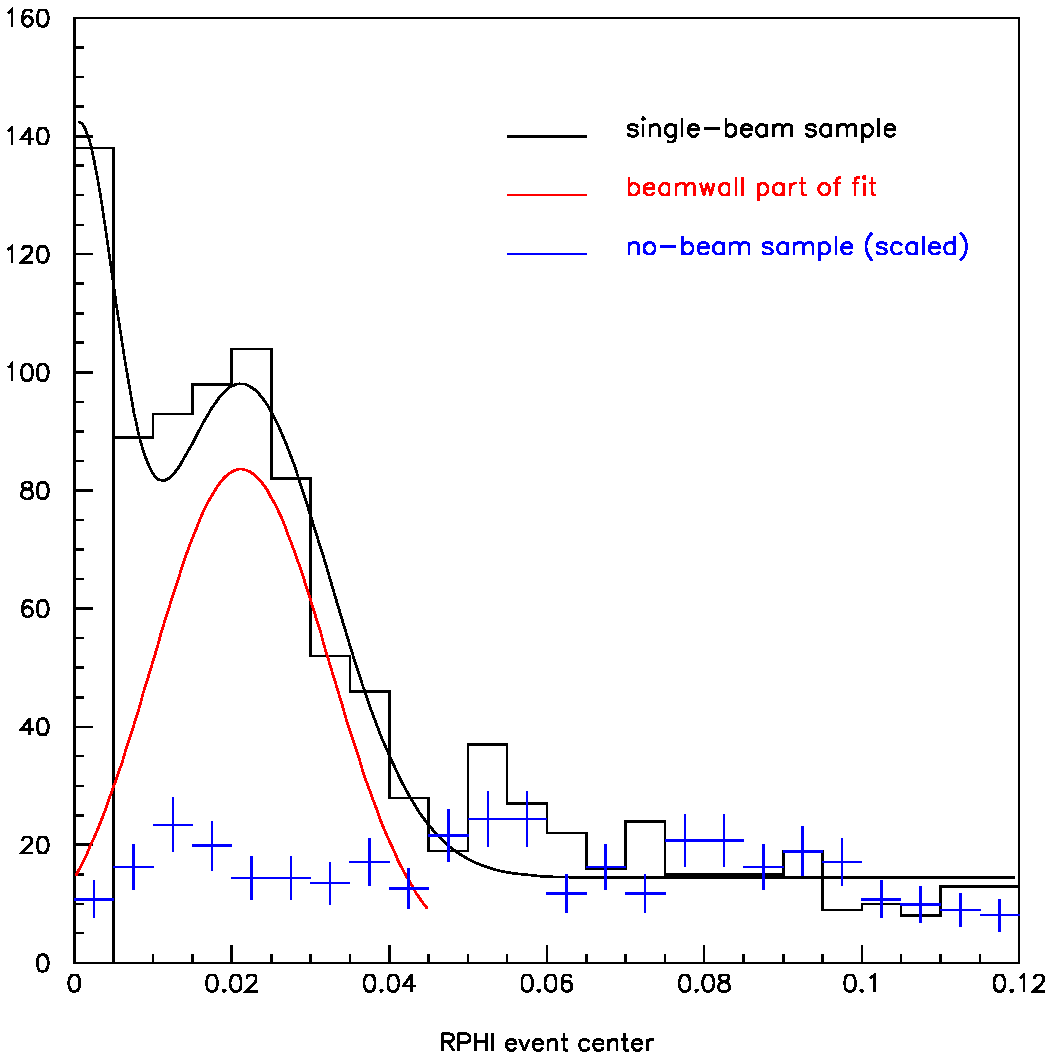
\includegraphics[width=0.8\linewidth]{old-school-histograms.pdf}}\only<2>{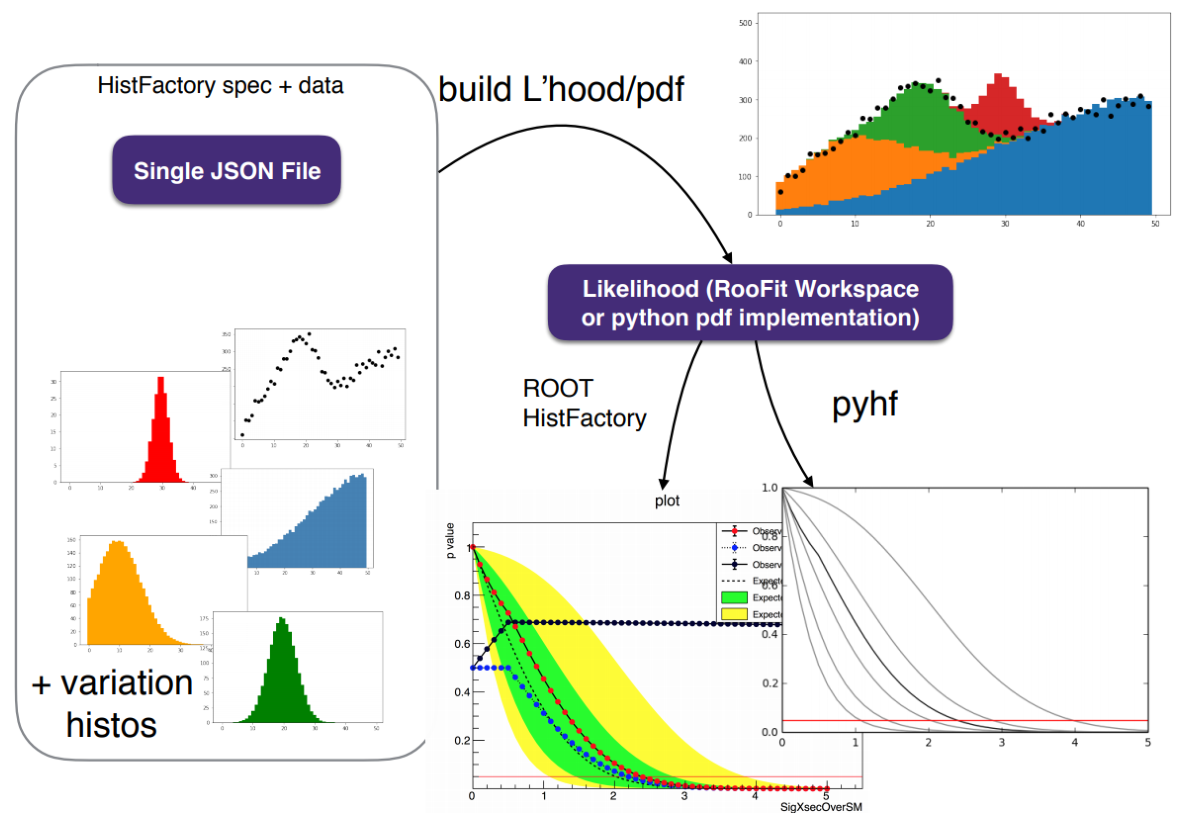
\includegraphics[width=\linewidth]{modern-histograms.pdf}}

\end{columns}
\end{frame}

\begin{frame}{Vague statement of the problem}
\vspace{0.5 cm}
\Large
\textcolor{darkblue}{A ``superhistogram'' is a large collection of histograms that are meant to be interpreted together.}
\end{frame}

\begin{frame}{Vague statement of the problem}
\vspace{0.5 cm}
\large

\textcolor{darkblue}{Representing a superhistogram with a directory of ordinary histograms is}

\vspace{0.5 cm}
\begin{itemize}\setlength{\itemsep}{0.5 cm}
\item \textcolor{darkblue}{wasteful} because much of the same metadata is copied in memory or on disk, and many small buffers of bin contents is less efficient than one big buffer.

\item \textcolor{darkblue}{inconvenient} because the object with a common meaning has to be managed as individual objects without an explicit connection. (Usually, they're linked with naming conventions.)
\end{itemize}
\end{frame}

\begin{frame}{Vague statement of the problem}
\vspace{0.5 cm}
\Large
\textcolor{darkblue}{Boost::Histogram provides a generic way to create an $n$-dimensional space with regular, variable, and categorical axes.}

\vspace{0.5 cm}
\begin{columns}
\column{0.6\linewidth}
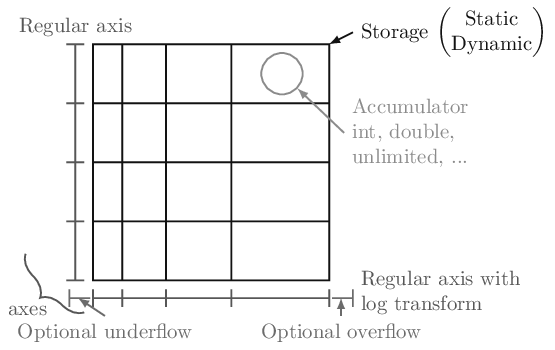
\includegraphics[width=\linewidth]{histogram_design.png}

\column{0.4\linewidth}
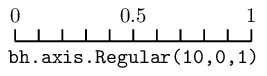
\includegraphics[width=\linewidth]{axis_regular.png}

\vspace{0.35 cm}
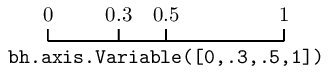
\includegraphics[width=\linewidth]{axis_variable.png}

\vspace{0.35 cm}
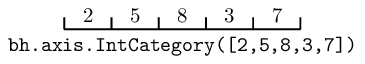
\includegraphics[width=\linewidth]{axis_category.png}
\end{columns}
\end{frame}

\begin{frame}{Vague statement of the problem}
\vspace{0.5 cm}
\Large

\textcolor{darkblue}{But a Boost::Histogram is still a single histogram:}

\vspace{0.25 cm}
\begin{itemize}
\item $n$ axes form an $n$-dimensional space,
\item each scalar \mintinline{python}{fill} operation increments {\it one} bin in that space.
\end{itemize}

\vspace{0.75 cm}
\begin{uncoverenv}<2->
\textcolor{darkblue}{A superhistogram has multiple sources, channels, and systematics.}

\vspace{0.25 cm}
\begin{itemize}
\item Not all histograms in the collection have the same number of bins or the same dimensions.
\item One \mintinline{python}{fill} of the superhistogram would increment every histogram in the collection.
\end{itemize}
\end{uncoverenv}
\end{frame}

\begin{frame}[fragile]{Something like this}
\vspace{0.15 cm}
\small
\begin{minted}{python}
h = SuperHist(SuperHist(
        SuperHist(
            Hist.new.Reg(100, 0, 30, name="syst-up"),
            Hist.new.Reg(100, 0, 30, name="nominal"),
            Hist.new.Reg(100, 0, 30, name="syst-down"),
            name="pt",
        ),
        SuperHist(
            Hist.new.Reg(50, -5, 5, name="syst-up"),
            Hist.new.Reg(50, -5, 5, name="nominal"),
            Hist.new.Reg(50, -5, 5, name="syst-down"),
            name="eta",
        ),
        name="data",
    ),
    ...,   # similarly for name="mc"
)
h.fill(pandas_dataframe)   # one row is a scalar fill operation
\end{minted}
\end{frame}

\begin{frame}{So far, this is looking like Histogrammar}
\vspace{0.08 cm}
\begin{center}
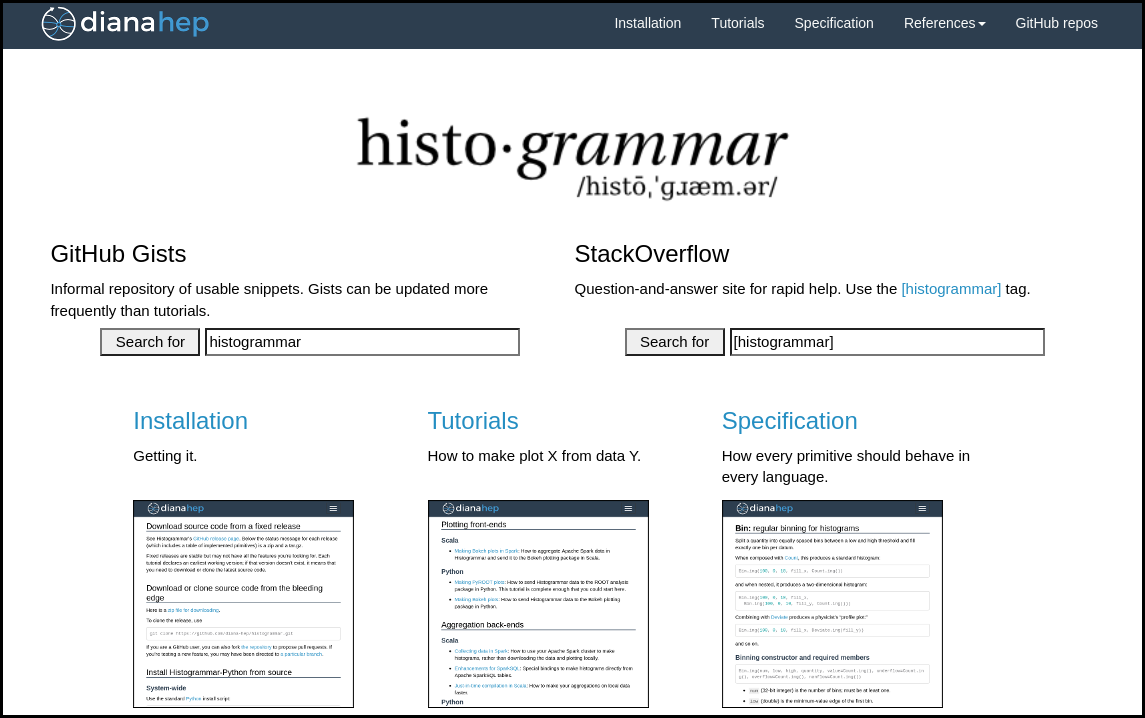
\includegraphics[width=0.9\linewidth]{histogrammar-website.png}
\end{center}
\end{frame}

\begin{frame}{R.I.P. Histogrammar}
\vspace{0.5 cm}
\Large
\textcolor{darkblue}{Histogrammar was too loose: it described a {\it tree} of nested binnings (unlike Boost::Histogram's {\it sequence}), and then there was no connection among the branches of the tree.}

\vspace{1 cm}
\uncover<2->{\textcolor{darkblue}{We need a relationship that restricts the superhistogram to a useful subset of all possible trees.}}
\end{frame}

\begin{frame}{Abstract algebra for fun (profit comes later)}
\vspace{0.5 cm}
\large

\textcolor{darkblue}{Many operations on data structures can be described as abstract algebras.}

\vspace{0.5 cm}
\begin{uncoverenv}<2->
The most common is a {\bf monoid}, which is any set $S$ with a binary operation $x \cdot y = z$ ($x \in S$, $y \in S$, $z \in S$) that

\begin{center}
\begin{minipage}{0.5\linewidth}
\begin{itemize}
\item[\textcolor{black}{\bf is associative:}] $(x \cdot y) \cdot z = x \cdot (y \cdot z)$

\item[\textcolor{black}{\bf has an identity:}] there is an $e \in S$ such that $e \cdot x = x$ and $x \cdot e = x$ for all $x \in S$.
\end{itemize}
\end{minipage}
\end{center}
\end{uncoverenv}

\vspace{0.5 cm}
\uncover<3->{\textcolor{gray}{(You may be familiar with {\bf groups}, which are {\bf monoids} without inverses.)}}
\end{frame}

\begin{frame}{Examples of monoids}
\large
\vspace{0.5 cm}

\begin{itemize}\setlength{\itemsep}{0.25 cm}
\item<1-> Natural numbers ($\Bbb{N} = \{0, 1, 2, \ldots\}$) under addition ($+$). The identity is $0$.
\item<2-> Positive integers ($\Bbb{P} = \{1, 2, \ldots\}$) under multiplication ($\times$). The identity is $1$.
\item<3-> Extended reals ($\Bbb{R} \times \{-\infty, \infty\}$) under minimization. The identity is $\infty$.
\item<4-> Strings (e.g. \mintinline{python}{"abc"}, \mintinline{python}{"def"}) under concatenation (e.g. \mintinline{python}{"abc" + "def"} $\to$ \mintinline{python}{"abcdef"}). The identity is the empty string (\mintinline{python}{""}).
\item<5-> Histogram contents with identical binning under histogram-addition (\mintinline{bash}{hadd}). The identity is the empty histogram. We can parallelize histogram-filling because adding bin contents is associative: we get the same answer no matter how \mintinline{python}{fill} operations are divided up among workers.
\item<6-> Boost::Histogram axes under Cartesian product: $n$ axes, an $n$-dimensional space, combined with $m$ axes, an $m$-dimensional space, forms an $(n + m)$-dimensional space. An axis with 1 bin could be called an identity.
\end{itemize}
\end{frame}

\begin{frame}{For superhistograms, we need a semiring}
\large
\vspace{0.5 cm}

A {\bf semiring} is any set $S$ with two operations, ``$+$'' and ``$\times$'', such that

\vspace{0.25 cm}
\begin{center}
\begin{minipage}{0.9\linewidth}
\begin{itemize}
\item $S$ under $+$ is a monoid; let's call its identity ``$0$''.
\item $S$ under $\times$ is a monoid; let's call its identity ``$1$''.
\item $+$ is commutative: \fbox{$a + b = b + a$}.
\item $0$ absorbs everything under $\times$: \fbox{$a \times 0 = 0 = 0 \times a$}.
\item $\times$ is distributive over $+$: \fbox{$a \times (b + c) = (a \times b) + (a \times c)$} \\ \hfill and \fbox{$(b + c) \times a = (b \times a) + (c \times a)$}.\mbox{\hspace{1.525 cm}}
\end{itemize}
\end{minipage}
\end{center}

\vspace{0.5 cm}
\uncover<2->{Example: natural numbers under ordinary addition and multiplication.}
\end{frame}

\begin{frame}[fragile]{Superhistograms as a semiring}
\large
\vspace{0.5 cm}

To build a superhistogram, we put axes together in two ways:

\vspace{0.25 cm}
\begin{itemize}
\item Cartesian product $\times$, to form a space, like an ordinary Boost::Histogram.
\item Collection $+$, to form a set, like a directory of histograms.
\end{itemize}

\vspace{0.5 cm}
\begin{uncoverenv}<2->
\begin{columns}
\column{1.05\linewidth}

\small
\begin{minted}{python}
StrCategory(["data", "mc"], name="src") * (
    Reg(100, 0, 30, name="pt") + Reg(50, -5, 5, name="eta")
)
\end{minted}

\vspace{-0.1 cm}
\centering {\normalsize is equal to}

\begin{minted}{python}
StrCategory(["data", "mc"], name="src") * Reg(100, 0, 30, name="pt") +
StrCategory(["data", "mc"], name="src") * Reg(50, -5, 5, name="eta")
\end{minted}

\vspace{0.1 cm}
\centering {\normalsize Two histograms have the same categorical axis, different regular axes.}
\end{columns}
\end{uncoverenv}
\end{frame}

\begin{frame}{Checking the properties}
\vspace{0.5 cm}
\large

\begin{itemize}\setlength{\itemsep}{0.25 cm}
\item<1-> Superhistograms under $+$ is a commutative monoid: a set of histograms has no intrinsic order and all lives at one level (no subdirectories).
\item<1-> The identity of $+$ is the empty set (no histograms).
\item<2-> Superhistograms under $\times$ is a monoid: an $n$-dimensional space $\times$ an $m$-dimensional space forms an $(n + m)$-dimensional space.
\item<2-> The identity of $\times$ is a one-bin axis.
\item<3-> $+$ and $\times$ obey a distributive property: if $a$, $b$, and $c$ are axes,

\vspace{-0.25 cm}
\[ a \times (b + c) = (a \times b) + (a \times c) \]

represents two 2-dimensional histograms, both with the same first axis $a$, differing in their second axes $b$ or $c$.
\end{itemize}
\end{frame}

\begin{frame}{A superhistogram is a jagged array}
\vspace{0.25 cm}
\large
In Boost::Histogram terms, axes $a$, $b$, and $c$ in expressions like

\vspace{-0.2 cm}
\[ a \times (b + c) = (a \times b) + (a \times c) \]

\vspace{0.2 cm}
would share one \mintinline{python}{Storage}, such as \mintinline{python}{Double} (an floating-point array).

\begin{center}
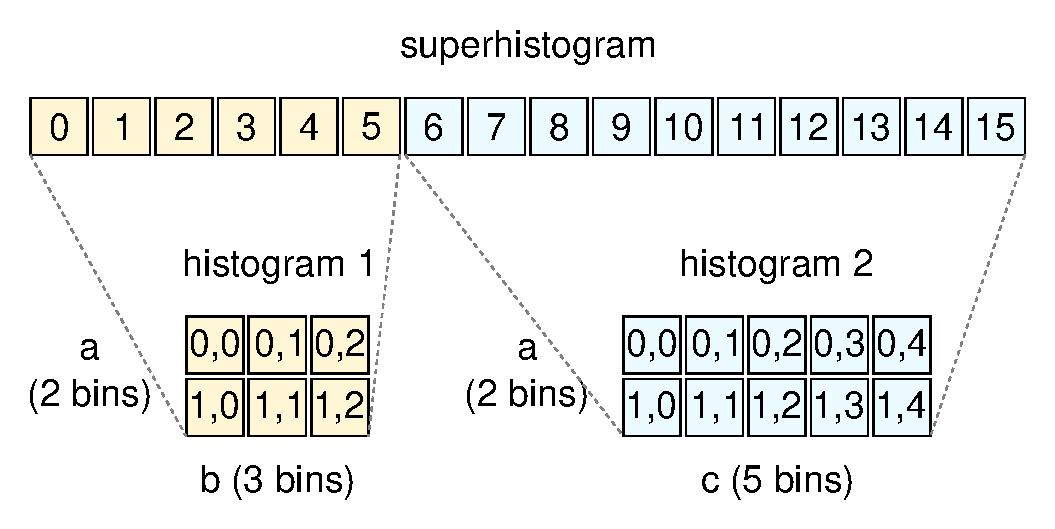
\includegraphics[width=0.8\linewidth]{sharing-storage.pdf}
\end{center}
\end{frame}

\begin{frame}[fragile]{A superhistogram is filled by DataFrames}
\vspace{0.25 cm}
\large

Each \mintinline{python}{fill} operation increments 1 bin in each multiplicative space, and every such space in an additive collection.

\small
\begin{minted}{python}
h = StrCategory(["data", "mc"], name="src") * (
    Reg(100, 0, 30, name="pt") + Reg(50, -5, 5, name="eta")
)
\end{minted}

\begin{columns}
\column{0.45\linewidth}
\hfill\mintinline{python}{h.fill(}

\column{0.2\linewidth}
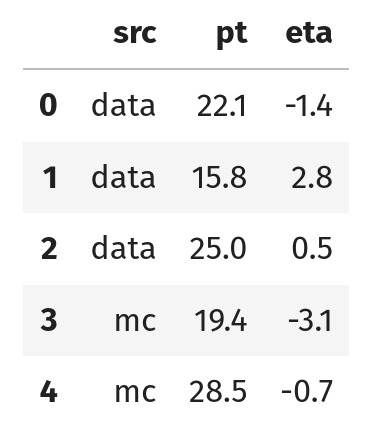
\includegraphics[width=\linewidth]{dataframe.png}

\column{0.45\linewidth}
\mintinline{python}{)}

\end{columns}

\large
\vspace{0.5 cm}
fills the histogram with axes \mintinline{python}{"src"} and \mintinline{python}{"pt"} 5 times, and \\ fills the histogram with axes \mintinline{python}{"src"} and \mintinline{python}{"eta"} 5 times.
\end{frame}

\begin{frame}{Abstract algebra for profit}
\vspace{0.5 cm}
\Large
\textcolor{darkblue}{Why does it matter that superhistograms form a semiring?}
\end{frame}

\begin{frame}{}

\end{frame}

\end{document}
